\documentclass[11pt]{scrartcl}
\usepackage[sexy]{evan}
\author{Konrad Kaczmarczyk}
\usepackage{amsmath,systeme}
\usepackage{listings}
\usepackage[T1]{fontenc}
\usepackage{graphicx}
\begin{document}
  \title{JAiO zima 2024}
  \subtitle{Rozwiązanie zadań z serii I}
  \maketitle
    \begin{zadanie}
        Dla dwóch języków $L, K$ nad alfabetem $\sum$, definiujemy język zawierający te podciągi słów z $L$, które można otrzymać poprzez równoczesne usunięcie rozłącznych infiksów, prefiksu i sufiksu, należących do $K$:
        \begin{gather*}
          L \ominus K = \{ v_1 v_2 \dots v_n \in \sum^* \mid v_{1}, v_{2}, \dots, v_n \in \sum^*, n \geq 1, \\
          \exists w_{0}, \dots , w_n \in K, w_0 v_{1} w_{1} v_{2} \dots  w_{n-1} v_n w_n \in L \}
        \end{gather*}
        Rozstrzygnij prawdziwość następujących zdań:
          \begin{walk}
              \item (1.5 pkt) Dla każdego $K$, jeśli $L$ jest regularny to $L \ominus K$ jest regularny.
              \item (1.5 pkt) Dla każdego $K$, jeśli $L \ominus K$ jest regularny to $L$ jest regularny.
              \item (2.0 pkt) Istnieje wielomian $p$ taki, że dla dowolnych języków $L$ i $K$, jeśli $L$ jest rozpoznawany przez automat deterministyczny o $n$ stanach, to $L \ominus K$ jest rozpoznawany przez automat deterministyczny o $p(n)$ stanach.
          \end{walk}
          
    \end{zadanie}

    \begin{walk}
    \item Tak, ustalmy dowolne $K \in \sum^*$, i dla dowolnego $L$ będącego regularne,  znamy jego automat $A(L)$. Pokażemy teraz że istnieje automat z $\varepsilon$-przejsciami rozpoznający $L \ominus K$. Aby go otrzymać do automatu $A(L)$ wprowadzimy nowy stan początkowy $q'_1$, oraz nowe stany końcowe $q'_{k_1}$, $q'_{k_2}$, itd., gdzie poprzednie stany końcowe już nimi nie są. Teraz wystarczy już wprowadzić nowe $\varepsilon$-przejscia, zadane wzorami:
      \begin{gather*}
        \forall_{q \in Q}\left ( q'_1, \varepsilon, q \right ) \in \delta \iff \exists_{w \in K} \left ( q_1, w, q \right ) \in \widehat{\delta} \\
      \forall_{q_n, q_m \in Q}\left ( q_n, \varepsilon, q_m \right ) \in \delta \iff \exists_{w \in K} \left ( q_n, w, q_m \right ) \in \widehat{\delta} \\
        \forall_{q, q'_{k_i} \in Q} \left ( q, \varepsilon, q'_{k_i} \right ) \in \delta \iff  \exists_{w \in K} \left ( q, w, q_{k_i} \right ) \in \widehat{\delta}
      \end{gather*}
     Zatem istnieje taki automat, a z wykładu wiemy że taki jest równoznaczny z jakims automatem deterministycznym, czyli $L \ominus K$ jest językiem regularnym.
        \item Nie, niech $K = a^*$, a $L = \{a^n | \; n \; \text{jest liczbą pierwszą} \}$, wtedy język $L \ominus K = a^*$, jest regularny, a sam $L$ nie jest (fakt ten pojawił się na ćwiczeniach).
        \item Nie, dowiedzmy to używając kontrprzykładu. Niech $L_n = (a + bc)^* c (a+c)^n$, i $K = b^*$. Do budowy automatu deterministycznego rozpoznającego język $L_n$, potrzebujemy dokładnie $4 + n$ klas, co udowodnimy indukcyjnie. Dla $n = 0$, wystarczą $4$ stany i automat wygląda tak,
          \begin{center}
            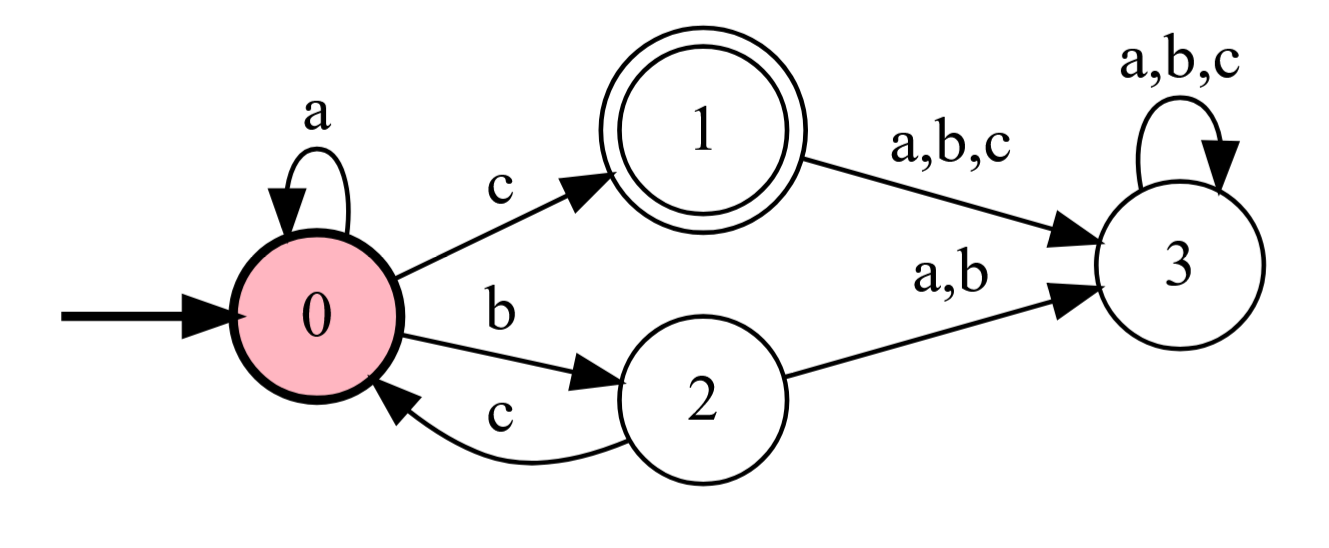
\includegraphics[width=10cm]{automat}
          \end{center}
          

          W przypadku kroku indukcyjnego wystarczy zmienić klasę końcową $c^n$ , na zwykłą i dodać nową klasę końcową $c^{n+1}$, zmienić parę przejsć, żeby otrzymać automat deterministyczny dla $L_{n+1}$. 
          Teraz rozpatrzmy automat dla $L_n \ominus K$, który generuje słowa dane wyrażeniem $(a+bc+c)^*c(a+c)^n$, który łatwo zauważyć że potrzebuje wykładniczo wiele stanów, bo słowa
          \begin{center}
              cc \dots ccc, cc \dots cca, cc \dots caa, cc \dots cac, itd.
          \end{center}
          są różnych klasach abstrakcji, zatem potrzebują osobnych stanów, a ich jest wykładniczo wiele (dokładnie $2^n$), wiemy że nie istnieje wielominan spełniający $p(n+4) > 2^n$, dla wszystkich $n$, co kończy dowód.
    \end{walk}
    
    
    
\end{document}
